%\documentclass{beamer}
\documentclass[handout]{beamer}
% This file is a solution template for:

% - Giving a talk on some subject.
% - The talk is between 15min and 45min long.
% - Style is ornate.

% Copyright 2004 by Till Tantau <tantau@users.sourceforge.net>.
%
% In principle, this file can be redistributed and/or modified under
% the terms of the GNU Public License, version 2.
%
% However, this file is supposed to be a template to be modified
% for your own needs. For this reason, if you use this file as a
% template and not specifically distribute it as part of a another
% package/program, I grant the extra permission to freely copy and
% modify this file as you see fit and even to delete this copyright
% notice. 


\mode<presentation>
{
  \usetheme{Montpellier}

  %\setbeamercovered{transparent}
  % or whatever (possibly just delete it)
}

\usepackage{xmpmulti} % package that defines \multiinclude

\usepackage[english]{babel}

\usepackage[latin1]{inputenc}

\usepackage{times}
\usepackage[T1]{fontenc}
% Or whatever. Note that the encoding and the font should match. If T1
% does not look nice, try deleting the line with the fontenc.

\title %[Vovk's algorithm] %(optional, use only with long paper titles)
{Tracking the best Expert}

\author[Freund] % (optional, use only with lots of authors)
{Yoav Freund}
% - Give the names in the same order as the appear in the paper.
% - Use the \inst{?} command only if the authors have different
%   affiliation.

\institute[Universities of Somewhere and Elsewhere] % (optional, but mostly needed)

\subject{Machine Learning}
% This is only inserted into the PDF information catalog. Can be left
% out. 

% If you have a file called "university-logo-filename.xxx", where xxx
% is a graphic format that can be processed by latex or pdflatex,
% resp., then you can add a logo as follows:

% \pgfdeclareimage[height=0.5cm]{university-logo}{university-logo-filename}
% \logo{\pgfuseimage{university-logo}}



% Delete this, if you do not want the table of contents to pop up at
% the beginning of each subsection:
%% \AtBeginSubsection[]
%% {
%%   \begin{frame}<beamer>
%%     \frametitle{Outline}
%%     \tableofcontents[currentsection,currentsubsection]
%%   \end{frame}
%% }


% If you wish to uncover everything in a step-wise fashion, uncomment
% the following command: 

\beamerdefaultoverlayspecification{<+->}

\newcommand{\newmcommand}[2]{\newcommand{#1}{{\ifmmode {#2}\else\mbox{${#2}$}\fi}}}
\newcommand{\renewmcommand}[2]{\renewcommand{#1}{{\ifmmode {#2}\else\mbox{${#2}$}\fi}}}
\newcommand{\newmcommandi}[2]{\newcommand{#1}[1]{{\ifmmode {#2}\else\mbox{${#2}$}\fi}}}
\newcommand{\newmcommandii}[2]{\newcommand{#1}[2]{{\ifmmode {#2}\else\mbox{${#2}$}\fi}}}
\newcommand{\newmcommandiii}[2]{\newcommand{#1}[3]{{\ifmmode {#2}\else\mbox{${#2}$}\fi}}}

\newcommand{\algfnt}{\bf}

\newmcommand{\ouralg}{{\mbox{\algfnt Hedge}({\eta})}}

\newmcommand{\iter}{T}

\newfont{\cmmib}{cmmib10}
\newcommand{\boldell}{{\mbox{\cmmib \symbol{'140}}}}


\newmcommandi{\costvec}{{\boldell}_{#1}}
\newmcommandii{\cost}{{\ell}^{#1}_{#2}}

\newmcommandi{\rd}{\tilde{#1}}

\newmcommandi{\distvec}{{\bf p}^{#1}}
\newmcommandi{\rddistvec}{\rd{\bf p}^{#1}}
\newmcommandii{\dist}{{p}^{#1}_{#2}}
\newmcommandii{\rddist}{\rd{p}^{#1}_{#2}}

\newmcommandi{\bdistvec}{{\bf q}^{#1}}
\newmcommandii{\bdist}{{q}^{#1}_{#2}}

\newmcommandi{\wtvec}{{\bf w}^{#1}}
\newmcommandi{\rdwtvec}{\rd{\bf w}^{#1}}
\newmcommandii{\wt}{{w}^{#1}_{#2}}
\newmcommandii{\rdwt}{\rd{w}^{#1}_{#2}}


\newcommand{\Nweight}[2]{V_{#1}^{#2}}	%the normalized weight
\newcommand{\dweight}[2]{w^{#2}(#1)} % initial density measure
\newcommand{\TEloss}[1]{L_{#1}}	%total loss of expert i
\newcommand{\BEloss}{L_{\min}}	%total loss of the best expert
\newcommand{\TAloss}{L_A}	%total loss of algorithm
\newcommand{\weight}[2]{W_{#1}^{#2}} % weight assigned to expert
\newcommand{\btheta}{\hat{\theta}}

\newcommand{\R}[1]{{\color{red}{#1}}}
\newcommand{\B}[1]{{\color{blue}{#1}}}
\newcommand{\RM}[1]{{\color{red}{$#1$}}}


%BANDITS
\newcommand{\Aplay}{{\bf Hedge}}
\newcommand{\Aest}{{\bf Exp3}}
\newcommand{\Aesthp}{{\bf Exp3.P}}
\newcommand{\Aestg}{{\bf Exp3.P.1}}
\newcommand{\Aests}{{\bf Exp3.S}}
\newcommand{\Aessg}{{\bf Exp3.S.1}}
\newcommand{\Astrat}{{\bf Exp4}}
\newcommand{\Abound}{{\bf Exp3.1}}
\newcommand{\Gbest}{G_{\rm max}}

\newcommand{\defeq}{\stackrel{\rm def}{=}}
\newcommand{\compl}{\mbox{\sc h}}
\newcommand{\theset}[2]{\{ {#1} \,:\, {#2} \}}

\newmcommandii{\stratv}{\mbox{\boldmath $\xi$}^{#1}({#2})}

%Games paper
\newmcommand{\M}{\bf M}
\newmcommand{\dM}{\M'}
\newmcommand{\Row}{\bf R}
\newmcommand{\dRow}{\R'}
\newmcommand{\C}{\bf C}
\newmcommand{\dC}{\C'}
\newmcommand{\D}{D}
\renewmcommand{\P}{\bf P}
\newmcommand{\Q}{\bf Q}
\newmcommand{\Dt}{\D_t}
\newmcommand{\Pt}{\P_t}
\newmcommand{\Qt}{\Q_t}
\newmcommand{\Pstar}{\P^*}	% the min/max optimal mixed strategy
\newmcommand{\Pref}{\tilde{\P}}	% a reference mixed strategy (not
				% necessarily min/max)
\newmcommand{\Qstar}{\Q^*}
\newmcommand{\Pa}{\overline{\P}}
\newmcommand{\Qa}{\overline{\Q}}
\newmcommand{\Qh}{\hat{\Q}}
\newmcommandi{\trans}{{#1}^{\rm T}}
\newmcommand{\mhx}{\M(h,x)}
\newmcommand{\mxh}{\dM(x,h)}
\newmcommand{\mpq}{\M(\P,\Q)}
\newmcommand{\mpsq}{\M(\Pstar,\Q)}
\newmcommand{\mpsqt}{\M(\Pstar,\Qt)}
\newmcommand{\mptqt}{\M(\Pt,\Qt)}
\newmcommand{\mptt}{\M(\Pt,t)}
\newmcommand{\mptq}{\M(\Pt,\Q)}
\newmcommand{\mpqt}{\M(\P,\Qt)}
\newcommand{\minp}{\min_{\P}}
\newcommand{\maxq}{\max_{\Q}}
\newcommand{\RE}[2]{{\rm RE}\left( {#1} \; \parallel \; {#2} \right) }

\newmcommand{\sumt}{\sum_{t=1}^T}
\newmcommand{\sumin}{\sum_{i=1}^n}
\newmcommand{\delt}{\Delta_{T,n}}
\newcommand{\nextline}{\vspace{0.2cm}\\}   % a little space for equation arrays

\newcommand{\lwalg}{\mbox{\rm MW}}
\newcommand{\lwalgvar}{\mbox{\rm vMW}}

%%
\newcommand{\E}{\mbox{\rm\bf E}}
\newcommand{\p}[2]{p_{#1}(#2)}
\newcommand{\q}[2]{q_{#1}(#2)}
\newcommand{\x}[2]{x_{#1}({#2})}
\newmcommand{\bx}{\mbox{\boldmath$x$}}
\newmcommandi{\xv}{\bx({#1})}
\newmcommand{\xvt}{\xv{t}}
%\newcommand{\w}[2]{w_{#1}({#2})} replaced by \wt, but remember to switch order of parameters i and t
\renewcommand{\i}[1]{i_{#1}}
\newcommand{\hx}[2]{\hat{x}_{#1}(#2)}
\newcommand{\hxit}{\hx{\i{t}}{t}}
\newcommand{\pit}{\p{\i{t}}{t}}
\newcommand{\xit}{\x{\i{t}}{t}}
\newcommand{\expb}[1]{\exp\left(#1\right)}

\newcommand{\vp}{{\mathbf p}}
\newcommand{\vu}{{\mathbf u}}
\newcommand{\vv}{{\mathbf v}}
\newcommand{\vx}{{\mathbf x}}
\newcommand{\vy}{{\mathbf y}}
\newcommand{\vw}{{\mathbf w}}
\newcommand{\vq}{{\mathbf q}}

\newcommand{\vecq}{{\bf q}}
\newcommand{\vecp}{{\bf p}}


\newcommand{\HedgeLoss}{L_{\mbox{\footnotesize Hedge}}}

\newcommand{\W}{\vec{W}}
\newcommand{\V}{\vec{V}}
\newcommand{\X}{\vec{X}}
\newcommand{\vb}{\vec{b}}
%\newcommand{\loss}{\vec{\ell}}
\newcommand{\loss}{L}
\newcommand{\elloss}[2]{\ell_{#2}\left( #1 \right)} %loss of expert i at time t
\newcommand{\lossvec}[1]{{\mathbf \ell}_{#1}}       %loss of expert at time t
\newcommand{\w}[1]{\makebox[12pt]{{#1}}}
\newcommand{\Rps}{\mbox{\tt R}}
\newcommand{\rPs}{\mbox{\tt P}}
\newcommand{\rpS}{\mbox{\tt S}}
\newcommand{\rpstie}{\w{$\frac{1}{2}$}}
\newcommand{\rpswin}{\w{$0$}}
\newcommand{\rpsloss}{\w{$1$}}

\newmcommand{\decspace}{\Delta}
\newmcommand{\decsym}{\delta}
\newmcommandi{\dec}{\decsym^{#1}}
\newmcommand{\decdistsym}{\cal D}
\newmcommandi{\decdist}{{\decdistsym}^{#1}}

\newmcommand{\simpdistspace}{{\bf \cal S}}
\newmcommand{\domset}{{\rm dom}(\decdistsym)}

\newmcommand{\expdistsym}{{\cal E}}
\newmcommandii{\expdist}{{\expdistsym}^{#1}_{#2}}
\newmcommand{\expdecsym}{{\varepsilon}}
\newmcommandii{\expdec}{\expdecsym^{#1}_{#2}}

\newmcommand{\outspace}{\Omega}
\newmcommand{\outsym}{\omega}
\newmcommandi{\out}{\outsym^{#1}}

%\newmcommandii{\Dkl}{D_{\mbox{kl}}\paren{#1||#2}}
\newmcommandii{\Dkl}{{\rm {KL}}\paren{{#1}\;||\;{#2}}}

\newmcommandi{\sumwts}{\sum_{i=1}^N \wt{#1}{i}}

\newmcommand{\lossalg}{L_A}
\newmcommand{\lossouralg}{{L_{\mbox{\scriptsize\algfnt Hedge}(\eta)}}}
\newmcommand{\lossS}{{L_{\mbox{\scriptsize\algfnt S}}}}
\newmcommandi{\lossi}{L_{#1}}
\newmcommandii{\lossit}{L_{#1}^{#2}}

\newmcommandi{\upbnd}{\tilde{#1}}

\newcommand{\angles}[1]{{\left\langle {#1} \right\rangle}}
\newcommand{\paren}[1]{{\left( {#1} \right)}}
\newcommand{\brac}[1]{{\left[ {#1} \right]}}
\newcommand{\braces}[1]{{\left\{ {#1} \right\}}}

\newcommand{\abs}[1]{{\left| {#1} \right|}}
\newcommand{\ceiling}[1]{{\left\lceil {#1} \right\rceil}}

\newfont{\msym}{msbm10}
\newcommand{\real}{\mbox{\msym R}}

\newmcommand{\updatefcn}{U_\eta}

%% \newtheorem{theorem}{Theorem}	
%% \newtheorem{lemma}[theorem]{Lemma}
%% \newtheorem{corollary}[theorem]{Corollary}
%% \newtheorem{definition}{Definition}

%\newcommand{\proof}{\noindent{\bf Proof:} }
%\newcommand{\example}[1]{{\em Example #1.} }
%\newcommand{\qed}{\rule{0.7em}{0.7em}}

\newcommand{\WeakAlg}{\mbox{\algfnt WeakLearn}}
\newcommand{\Boost}{\mbox{\algfnt AdaBoost}}
\newcommand{\EX}{\mbox{\bf EX}}
\newmcommand{\hf}{h_{{f}}}
\newmcommand{\rdhf}{\rd{h}_{{f}}}
\newmcommand{\hfT}{h^T_{{f}}}
\newmcommand{\ranh}{{b}}

\newmcommand{\conclass}{{\cal C}}

\newmcommand{\badvec}{{\bf b}}
\newmcommandi{\bad}{{b}_{#1}}

%%%%%%%% New commands defined for the game-playing paper

\newmcommand{\hedge}{\algfnt Hedge}
\newmcommand{\play}{\algfnt Play}
\newmcommandi{\Glossvec}{{\bg y}^{#1}}
\newmcommandii{\Gloss}{{y}^{#1}_{#2}}
%\newmcommandi{\action}{{I}_{#1}}
\newmcommandi{\Gdistvec}{{\bf \tilde{p}}^{#1}}
\newmcommandii{\Gdist}{{\teilde{p}}^{#1}_{#2}}

%%%%%%%%%%%%%%%%%%%%%%%%%%%%%%%%%%%%%%%%%%%%%%%%%%%%%
\newmcommand{\Idistvec}{{D}}
\newmcommandi{\Idist}{\Idistvec({#1})}
\newmcommand{\Idistt}{\Idistvec_t}

\newmcommand{\Xdist}{{\cal P}}
\newmcommand{\emp}{\hat{\epsilon}}

\newmcommand{\classpc}{Y}
\newmcommand{\numclass}{k}
\newmcommandii{\prob}{\mbox{\rm Pr}_{#1}\left[{#2}\right]}
\newmcommandii{\exval}{\mbox{\rm E}_{#1}\left[{#2}\right]}

%\usepackage{amsmath}
\DeclareMathOperator*{\argmax}{argmax} % thin space, limits underneath in displays
\DeclareMathOperator*{\argmin}{argmin} 

\newcommand{\RR}{\mathbb{R}}
\newcommand{\regret}{\mbox{Regret}}

%%% Conditional probabilities
\newmcommandii{\condp}{p\left( #1 \left| #2 \right. \right)}

\newmcommand{\lab}{y}
\newmcommand{\ploss}{\mbox{ploss}}
\newmcommandii{\avploss}{\ploss_{#1}({#2})}
\newcommand{\sfrac}[2]{\mbox{$\frac{#1}{#2}$}}

\newcommand{\mboosta}{\mbox{\algfnt AdaBoost.M1}}
\newcommand{\mboostb}{\mbox{\algfnt AdaBoost.M2}}
\newcommand{\mboostr}{\mbox{\algfnt AdaBoost.R}}

%\newmcommand{\slos}{\mbox{ploss}}
%\newmcommandiii{\sloss}{\slos_{#1}({#2},{#3})}
%\newmcommandiii{\avsloss}{\slos_{{#1},{#2}}({#3})}

\newmcommandii{\vwt}{{W}^{#1}_{#2}}

\newcommand{\figline}{\rule{\textwidth}{1pt}}

%\newmcommandi{\1}{{\bf 1}({#1})}
\newmcommandi{\1}{[\![{#1}]\!]}

\newmcommand{\confcn}{\kappa}
\newmcommandi{\erint}{\abs{\int_{y_i}^{h_t(x_i)} {#1} dy}}
%\newmcommandi{\erint}{\int_{\min\{y_i,h_t(x_i)\}}^{\max\{y_i,h_t(x_i)\}}{#1}dy}


\begin{document}

\iffalse %%%%%%%%%%%%%%%%%%%%%%%%%%%%%%%%%%%%%%%%%%%%%%%%%%%%%%%%%%%%%%%%%%
\fi %%%%%%%%%%%%%%%%%%%%%%%%%%%%%%%%%%


\begin{frame}
  \titlepage
\end{frame}
\section{Homework}
\begin{frame}
\frametitle{HW 3} 
\begin{itemize}
\item Let $x \in \{0,1\}$ and let $y \in[0,1]$.
\item Show that log loss $x \log y + (1-x)\log(1-y)$ is mixable.
\item Show that square loss $(x-y)^2$ is mixable.
\item Show that absolute loss $|x-y|$ is not mixable.
\item HW 3 is due on Feb 18.
\item No class on Tues 11 (ALT)
\item There will be no mid-term exam.
\end{itemize}
\end{frame}

\section{Review}
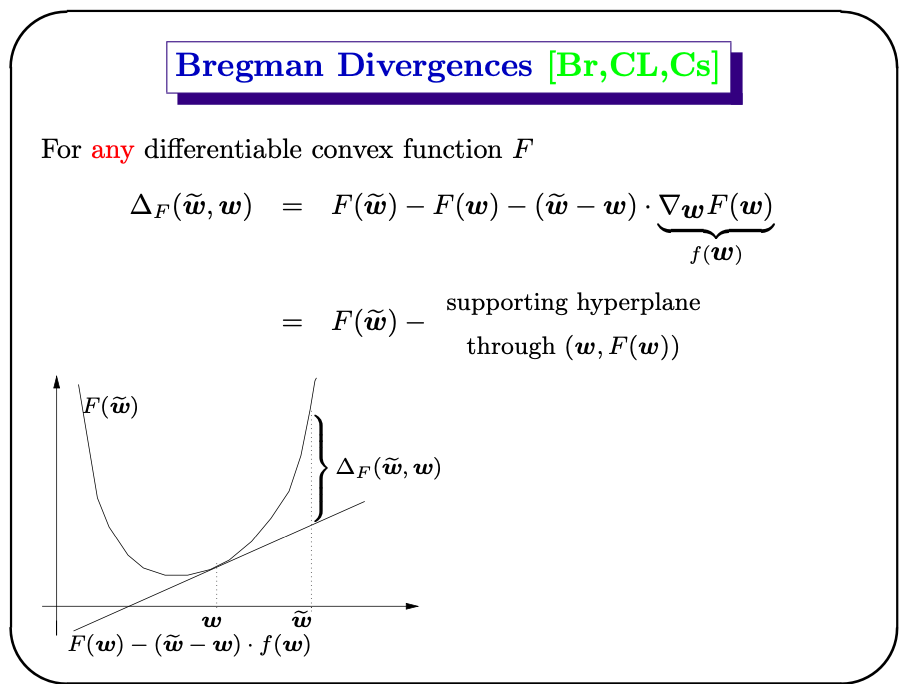
\includegraphics[width=4in]{ManfredSlides/skitch9.png}\\
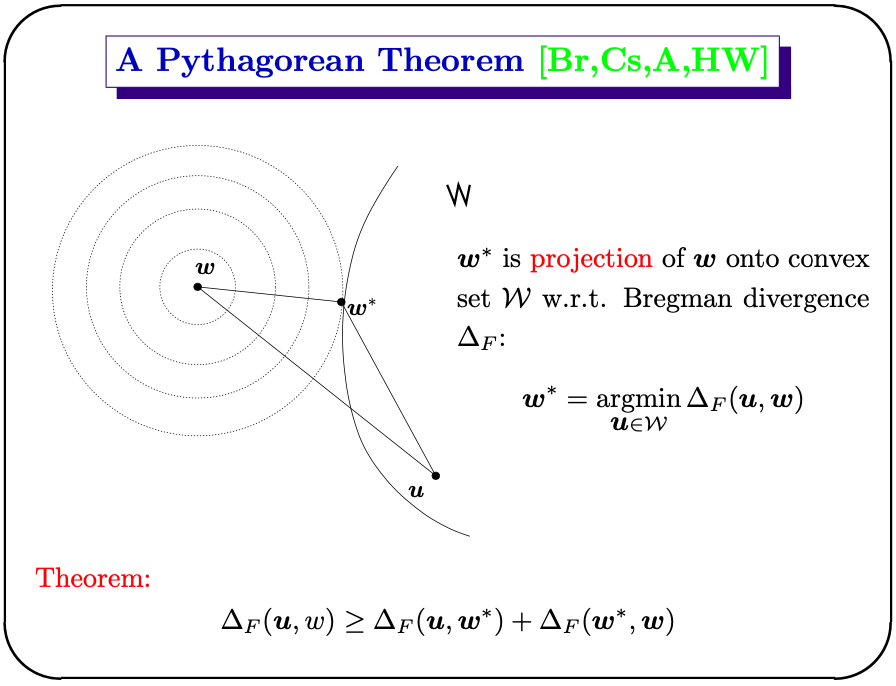
\includegraphics[width=4in]{ManfredSlides/skitch6.png}

\begingroup
\small
\begin{frame}
\frametitle{Unnormalized Relative entropy} 
\begin{itemize}
\item prediction, outcome \R{$\vecp,\vecq$} are \R{$n$} dimensional
  vectors with non-negative coordinates. 
\item Loss is RE extended to non-negative vectors:
\R{\[ \RE{\vecp}{\vecq} = \sum_{i=1}^n p_i \log \frac{p_i}{q_i} -
    \sum_{i=1}^n (q_i-p_i) \]}
Coincides with \R{RE} when \R{$\sum_{i=1}^n p_i = \sum_{i=1}^n q_i = 1$}
\item Unnormalized \R{RE} is the Bregman divergence corresponding to
  the unnormalized entropy:
  \R{\[
      F(\vecp) = \sum_{i=1}^n p_i \log p_i - \sum_{i=1}^n p_i
    \]}
\end{itemize}
\end{frame}

\begin{frame}
\frametitle{Inequalities for Unnormalized Relative entropy} 
\begin{itemize}
\item
\B{No} \B{triangle inequality}
\R{$ \exists \vecp_1,\vecp_2,\vecp_3\;\; \RE{\vecp_1}{\vecp_3} >
  \RE{\vecp_1}{\vecp_2} + \RE{\vecp_2}{\vecp_3}
$}
\item \B{Generalized Pythagorean inequality}
  For any closed convex set \R{$S$} and any point \R{$\vecp_1 \notin
    S$}, define the projection of \R{$\vecp_1$} on \R{$S$} to be
  \R{$\vecp_2 = \mbox{argmin}_{\vu \in S} \RE{\vecp_1}{\vu}$}, then:
  \R{\[
       \forall \vecp_3 \in S;\;\; \RE{\vecp_1}{\vecp_3} \geq \RE{\vecp_1}{\vecp_2} + \RE{\vecp_2}{\vecp_3}
\]}
\end{itemize}
\end{frame}

\begin{frame}
\frametitle{half squared euclidean distance}
\begin{itemize}
\item prediction, outcome \R{$\vu,\vv \in R^n$}
\item
  \R{\[ \lambda_{\text{sq}}(\vu,\vv)  = \frac{1}{2} \|\vu-\vv\|^2 =
      \frac{1}{2} \sum_{i=1}^n (u_i - v_i)^2
  \]}
\item
Bregman divergence with respect to the square euclidean norm
\R{$$\| \vv \|_2$$}
\item Triangle inequality does not hold.
\item \B{Pythagoras inequality} :
  For any closed convex set \R{$S$} and any point \R{$\vv_1 \notin
    S$}, define the projection of \R{$\vv_1$} on \R{$S$} to be 
  \R{$\vv_2 = \mbox{argmin}_{\vu \in S} \| \vv_1 - \vu \|^2$}, then:
  \R{\[
      \forall \vv_3 \in S;\;\; \| \vv_1 - \vv_3 \|^2 \geq \| \vv_1 - \vv_2 \|^2 + \| \vv_2 - \vv_3 \|^2
    \]}
\end{itemize}
\end{frame}
\endgroup

\begin{frame}
\frametitle{Bregman divergence regularization}
\begin{itemize}
\item Idea: Set $\vw_{t+1}$ to be  \R{$\vu$} that minimizes:
  \R{\[
       \Delta_F(\vw_t,\vu) + \alpha \costvec{t}(\vu) 
  \]}
\item In general, hard to compute the minimum.
\item Efficient approximation \B{Mirror Descent}. Will be covered later.
\end{itemize}
\end{frame}

\section{Tracking linear experts}
\begin{frame}
\frametitle{Tracking Linear Experts }
\begin{itemize}
\item \B{Usually:} compare algorithm's total loss to total
  loss of the best expert.
\item \B{drifting experts:} Compare with a sequence of experts that
  change over time.
\item The amount of change is measured using total bregman
  divergence.
\item Regret depends on \R{$\sum_t \Delta_F(\vu_t-1,\vu_t)$}
\item \B{The Projection Update} After computing the unconstrained
  update, project the $\vw_{t+1}$ onto a convex set.
\item Does not allow the algorithm to over-commit to an extreme vector
  from which it is hard to recover.
\end{itemize}
\end{frame}


\section{Switching Experts}

\begin{frame}
\frametitle{Switching experts setup}
\begin{itemize}
\item \B{Usually:} compare algorithm's total loss to total
  loss of the best expert.
\item \B{Switching experts:} compare algorithm's total loss to total
  loss of \B{best expert sequence} with \R{$k$} \B{switches}.
\item
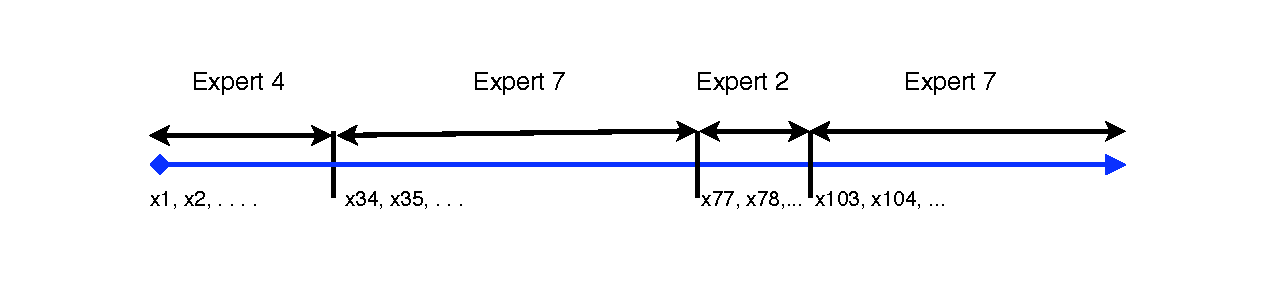
\includegraphics[width=4.5in]{figures/SwitchingExperts.pdf}
\end{itemize}
\end{frame}

\section{An inefficient algorithm}

\begin{frame}
\frametitle{An inefficient algorithm}
\begin{itemize}
\item Fix:
\begin{itemize}
\item \R{$l$} - sequence length
\item \R{$k$} - number of switches
\item \R{$n$} - number of experts
\end{itemize}
\item Consider one \B{partition-expert} per sequence of switching experts.
\item No. of \B{partition-expert}s : 
\R{${l \choose k-1} n (n-1)^k = O \paren{n^{k+1} \paren{\frac{el}{k}}^k} $}
\item The log-loss regret is at most 
\R{$(k+1) \log n + k \log \frac{l}{k} +k$}
\item Requires maintaining \R{$O \paren{n^{k+1} \paren{\frac{el}{k}}^k}$} weights.
\end{itemize}
\end{frame}

\begin{frame}
\frametitle{generalization to mixable losses}
\begin{itemize}
\item In this lecture we assume loss function is \B{mixable}.
\item There is an exponential weights algorithm with learning rate \R{$\eta$} that 
achieves (in the non-switching case) a bound 
\R{\[
L_A \leq \min_i L_i + \frac{1}{\eta} \log n
\]}
\item Then using the \B{partition-expert} algorithm for the switching-experts case 
we get a bound on the regret 
\R{$\frac{1}{\eta} \paren{(k+1) \log n + k \log \frac{l}{k} +k}$}
\end{itemize}
\end{frame}


\begin{frame}
\frametitle{Weight sharing algorithms}
\begin{itemize}
\item Update weights in two stages: loss update then share update.
\item Prediction uses the normalized \R{$s$} weights \R{$w_{t,i}^s / \sum_j w_{t,j}^s$}
\item \B{Loss update} is the same as always, but defines intermediate \R{$m$} weights:
\R{\[
w_{t,i}^m = w_{t,i}^s e^{-\eta L(y_t,x_{t,i})}
\]}
\item \B{Share update}: redistribute the weights
\item \B{Fixed-share}: 
\R{\begin{eqnarray*}
pool & = & \alpha \sum_{i=1}^n w_{t,i}^m \\
w_{t+1,i}^s & = & (1-\alpha) w_{t,i}^m + \frac{1}{n-1} \paren{pool - \alpha w_{t,i}^m}
\end{eqnarray*}}
\end{itemize}
\end{frame}

\section{The fixed-share algorithm}

\begin{frame}
\frametitle{The fixed-share algorithm}
\multiinclude[graphics={width=11cm},format=pdf]{figures/IntermediateWeights}
\end{frame}

\begin{frame}
\frametitle{Proving a bound on the fixed-share}
\begin{itemize}
\item The relation between algorithm loss and total weight does not change
because share update does not change the total weight.
\item Thus we still have 
\R{\[
L_A \leq \frac{1}{\eta} \sum_{i=1}^n w_{l+1,i}^s
\]}
\item The harder question is how to lower bound \R{$\sum_{i=1}^n w_{l+1,i}^s$}
\end{itemize}
\end{frame}

\begin{frame}
\frametitle{Lower bounding the final total weight}
\begin{itemize}
\item Fix some switching experts sequence:
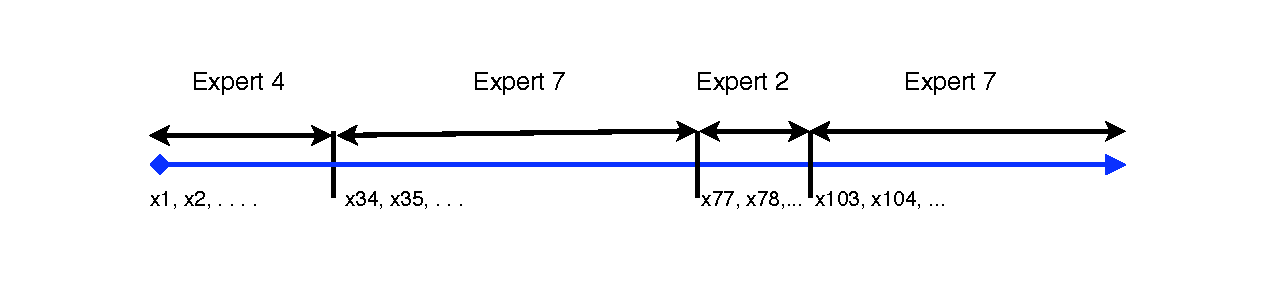
\includegraphics[width=4.5in]{figures/SwitchingExperts.pdf}
\item \B{``follow''} the weight of the chosen expert $i_t$.
\item The loss update reduces the weight by a factor of \R{$e^{-\eta \ell_{t,i_t}}$}.
\item The share update reduces the weight by a factor larger than:
\begin{itemize}
\item \R{$1-\alpha$} on iterations with no switch.
\item \R{$\frac{\alpha}{n-1}$} on iterations where a switch occurs.
\end{itemize}
\end{itemize}
\end{frame}

\begin{frame}
\frametitle{Bound for arbitrary $\alpha$}
\begin{itemize}
\item
Combining we lower bound the final weight of the last expert in the sequence
\R{\[
w^s_{l+1,e_k} \geq \frac{1}{n} e^{-\eta L_*} (1-\alpha)^{l-k-1} \paren{\frac{\alpha}{n-1}}^k
\]}
Where \R{$L_*$} is the cumulative loss of the switching sequence of experts.
\item
Combining the upper and lower bounds we get that for any sequence 
\R{\[
L_A \leq L_* + 
\frac{1}{\eta} \paren{ \ln n + \paren{l-k-1} \ln \frac{1}{1-\alpha}
                       +k \paren{ \ln \frac{1}{\alpha} + \ln (n-1)}}
\]}
\end{itemize}
\end{frame}

\begin{frame}
\frametitle{Tuning $\alpha$}
\begin{itemize}
\item let \R{$k^*$} be the best number of switches (in hind sight) 
and \R{$\alpha^* = k^* / l$}
\item Suppose we use \R{$\alpha \approx \alpha^*$} then the bound that we get is
\R{\[
L_A \leq L_* + \frac{1}{\eta} \paren{(k+1) \ln n 
+ (l-1)\paren{H(\alpha^*) + D_{\text{KL}}(\alpha^* || \alpha)}}
\]}
Where
\R{
\[
H(\alpha^*) = -\alpha^* \ln \alpha^* - (1-\alpha^*) \ln (1-\alpha^*)
\]
\[
D_{\text{KL}}(\alpha^* || \alpha) = 
\alpha^* \ln \frac{\alpha^*}{\alpha}  (1-\alpha^*) \ln \frac{1-\alpha^*}{1-\alpha}
\]
}
\item This is very close to the loss of the computationally inefficient algorithm.
\item For the log loss case this is essentially optimal.
\item Not so for square loss!
\end{itemize}
\end{frame}

\section{The variable-share algorithm}

\begin{frame}
\frametitle{What can we hope to improve?}
\begin{itemize}
\item In the fixed-share algorithm, the 
weight of a suboptimal expert never decreases below
\R{$\alpha/n$}.
\item The algorithm does not concentrate only on the best expert, even
if the last switch is in the distant past.
\item The regret depends on the length of the sequence.
\end{itemize}
\end{frame}

\begin{frame}
\frametitle{The idea of variable-share}
\begin{itemize}
\item Let the fraction of the total weight given to the 
best expert get arbitrarily close to \R{$1$}.
\item we can get a regret bound that depends only on the number of
switches, not on the lenght of the sequence.
\item Requires that the loss be bounded.
\item Works for \B{square} loss, but not for \B{log} loss!
\end{itemize}
\end{frame}

\begin{frame}
\frametitle{Variable-share}
\R{\begin{eqnarray*}
pool & = & \sum_{i=1}^n \paren{1-\paren{1-\alpha}^{\ell_{t,i}}} w_{t,i}^m \\
w_{t+1,i}^s & = & (1-\alpha)^{\ell_{t,i}} w_{t,i}^m + 
\frac{1}{n-1} \paren{pool - \paren{1-\paren{1-\alpha}^{\ell_{t,i}}} w_{t,i}^m}
\end{eqnarray*}}
\pause
If \R{$\ell_{t,i} = 0$}, then expert \R{$i$} does not contribute to the pool.\\
\pause
Expert can get fraction of the total weight arbitrarily close to \R{$1$}.\\
\pause
Shares the weight quickly if \R{$\ell_{t,i}>0$}
\end{frame}

\begin{frame}
\frametitle{Bound for variable share}
\begin{itemize}
\item
\R{
\[
\frac{1}{\eta} \ln n +
\paren{ 1+ \frac{1}{(1-\alpha)\eta}} L_* +
k \paren{1 + \frac{1}{\eta} \paren{ \ln {n-1} + \ln \frac{1}{\alpha} + \ln \frac{1}{1-\alpha} }}
\]
}
\item \R{$\alpha$} should be tuned so that it is (close to) 
\R{$\frac{k}{2k+L_*}$}
\end{itemize}
\end{frame}

\begin{frame}
\frametitle{An experiment using variable share}
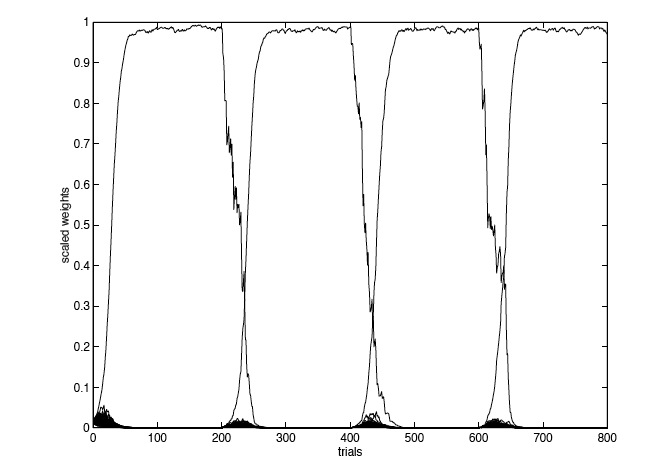
\includegraphics[height=6cm]{figures/VariableShareFigure.jpg}
\end{frame}

\begin{frame}
\frametitle{Switching within a small subset}
\begin{itemize}
\item Suppose the best switching sequence is repeatedly switching among a small subset of the experts
\R{$n' \ll n$}
\item In the context of speech recognition - the speaker repeatedly uses a small number of phonemes.
\item If we know the subset, we can pay \R{$\ln n'$} per switch rather than \R{$\ln n$}
\item Can track switches much more closely.
\item Easy to describe an inefficient algorithm (consider all \R{${n \choose n'}$} subsets.)
\item Switching to Slides from Manfred Warmuth.
\end{itemize}
\end{frame}

\iffalse %%%%%%%%%%%%%%%%%%%%%%%%%%%%%%%%%%%%%%%%%%%%%%%%%%%%%%%%%%%%%%%%%%

\fi %%%%%%%%%%%%%%%%%%%%%%%%%%%%%%%%%%

\end{document}


